%%%%%%%%%%%%%%%%%%%%%%%%%%%%%%%%%%%%%%%%%%%%%%%%%%%%%%%%%%%%%%%%%%%%%%%%%%%%%%%%%%%%%%%%%%
\section{Evaluation}
%%%%%%%%%%%%%%%%%%%%%%%%%%%%%%%%%%%%%%%%%%%%%%%%%%%%%%%%%%%%%%%%%%%%%%%%%%%%%%%%%%%%%%%%%%i
\subsection{Security: do we meet our meet security goals}
   - attack scenarios

\subsection{Performance}
We measure two aspects of \sys's performance: (1) the latency and storage cost of using \sys's
low-level API to apply a disguise, reveal a disguise, or temporarily recorrelate disguised data; and
(2) the impact of these disguising operations on the performance of concurrently executing
application users.

\lyt{TODO describe WebSubmit (or put case study first so we have the description?)}

\head{Cost of \sys's API.}
\begin{table}[t!]
\begin{center}
\begin{tabular}{ c c }
 \textbf{High-Level Operation} & \textbf{Time (mus)}\\
\hline
    Create User Account & 1000\\
    Delete User Account & 5250/lec\\
    Restore User Account & 18300/lec\\
    Anonymize User Account & 900/lec\\
    Edit Normal Lecture Answers & 2000/lec \\
    Edit Anonymized Lecture Answers & 62000/lec \\
\hline
    \textbf{DB Operation} & \textbf{Time (mus)}\\
\hline
Insert DB Row (User )& 120\\
Update DB Row (FK) & 64\\ 
Select DB Row (User) & 120\\
Remove DB Row (User) & 90\\
Select DB Rows (Answers) & 160\\
Remove DB Rows (Answers) & 150\\
Reveal Deleted Row (DB Select + Insert) & 160 \\
Create + Register Principal & 110\\
\hline
    \textbf{Crypto Operation} & \textbf{Time (mus)}\\
\hline
Generate Keypair & 300831\\
Encrypt Ownership Token & 360\\
Decrypt Ownership Token & 3000\\
Encrypt Diff Token & 340\\
Decrypt Diff Token & 3000\\
\end{tabular}
\end{center}
\caption{Amount of time required to run different operations for disguises in WebSubmit. Each
    lecture is associated with 4 answers.}
    \label{tab:opstats}
\end{table}

Table~\ref{tab:opstats} shows the latency of different operations involved in disguising. 
The latency of each high-level operation shown scales linearly with amount
of data (\ie number of lectures and answers per lecture) associated with the user,
and requires some number of DB or crypto operations.

Creating an account in WebSubmit generates an APIKey and registers a private-public keypair
for the user (returing the public key as the user's decryption capability).

Account deletion requires decrypting one ownership token for each lecture; selecting DB rows of
both the original principal and any linked pseudoprincipals to remove; removing these
selected rows; and encrypting and inserting one diff token for each answer for each lecture.

Account restoration requires decrypting a diff token for each answer for each lecture; DB queries to check
whether the diffs can be restored (\eg that the corresponding lecture of an answer to reinsert
still exists); and DB queries to restore the disguised data to its original state.

Account anonymization requires selecting the relevant answers to anonymize; generating
pseudoprincipals and ownership tokens for each answer; encrypting and storing these ownership tokens; and performing DB queries to actually update application data.

Editing answers of a lecture normally performs the relevant update DB queries. However, editing
anonymized answers of a lecture uses client-provided locator and decryption capabilities to
authorize the client to speak for the pseudoprincipal associated with the answer. \sys performs this
authorization check by decrypting \emph{all} ownership tokens at the specified locator with the
decryption capability until it finds a ownership token linking the client to the owning
pseudoprincipal. For example, anonymization of a user account with answers to 20 lectures generates
20 ownership tokens encrypted at the same locator; editing the answers of a single lecture thus
performs up to 20 decryptions to determine which pseudoprincipals the client can act for. This can
be optimized by batching all ownership tokens from one disguise into a single encrypted ciphertext.

\head{Impact on Normal Application Execution.}

\subsection{Case studies}
   1) websubmit
      - was Edna sufficient for the application's needs?
      - changes to application required (how much work to integrate Edna?)
      - *how* did application use Edna?
        - what disguises?
        - how caps integrated with application?
   2) HotCRP
   3) Lobsters?

\begin{figure*}[t!]
    \centering
    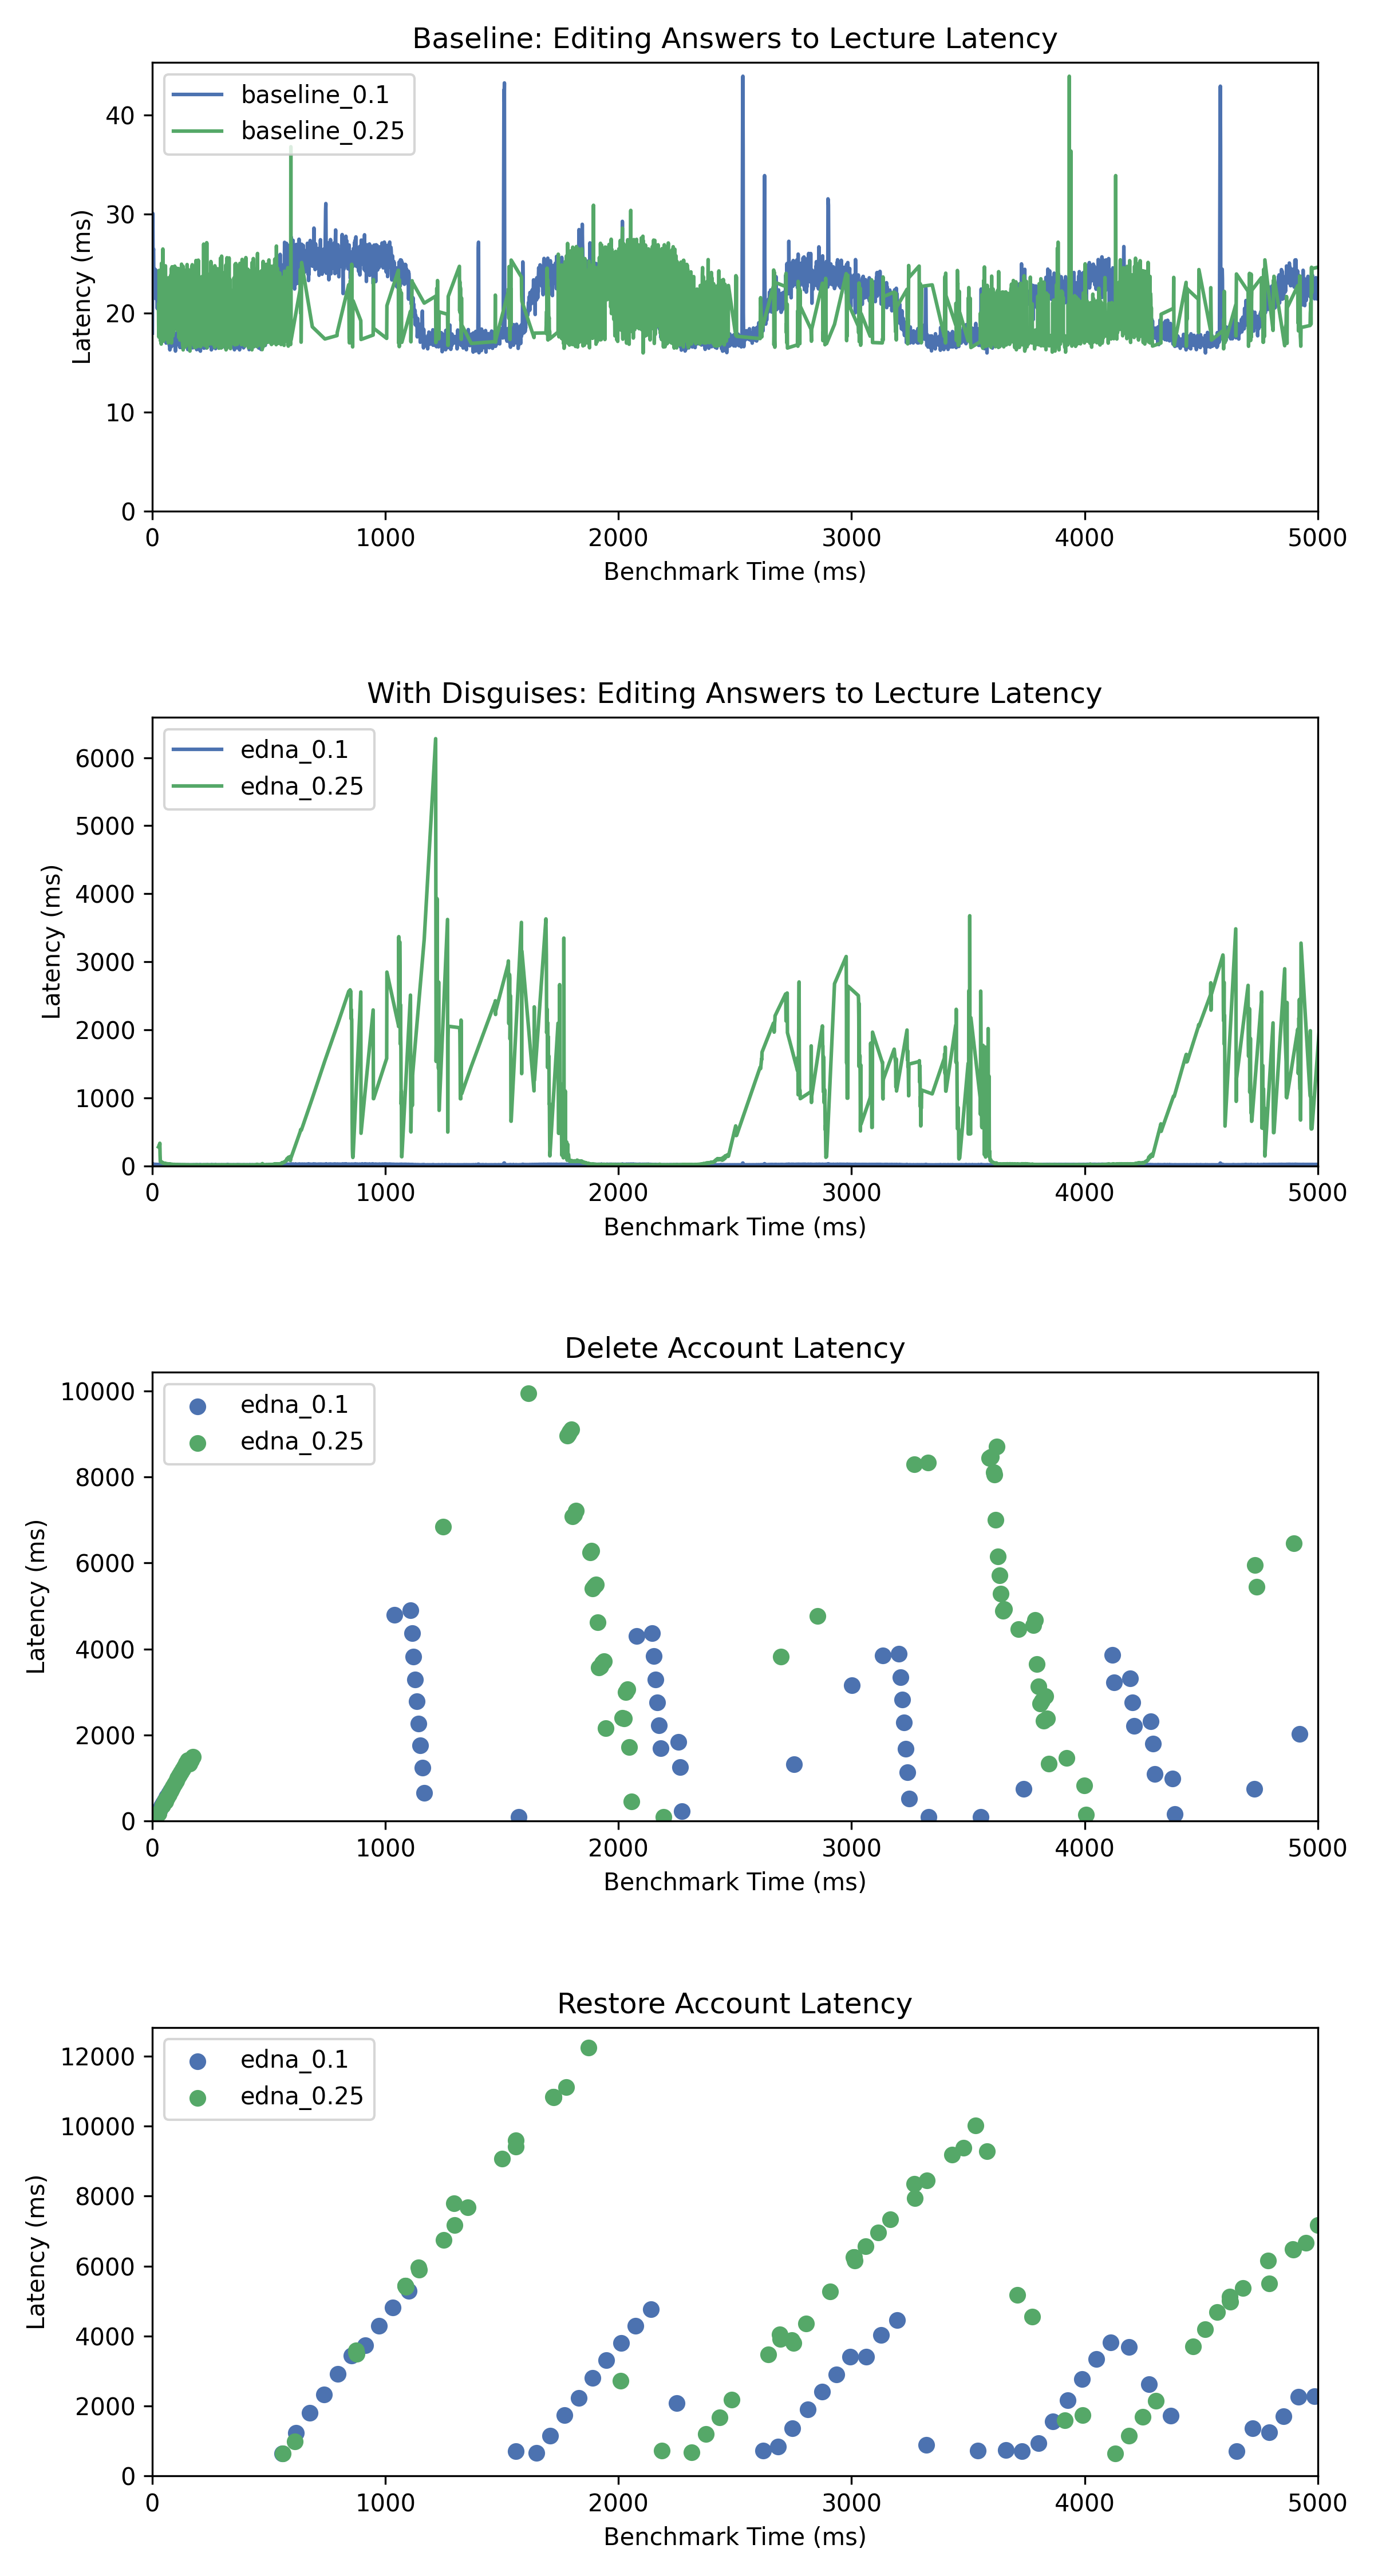
\includegraphics[width=0.45\textwidth]{figs/concurrent_results_40lec_100users}
    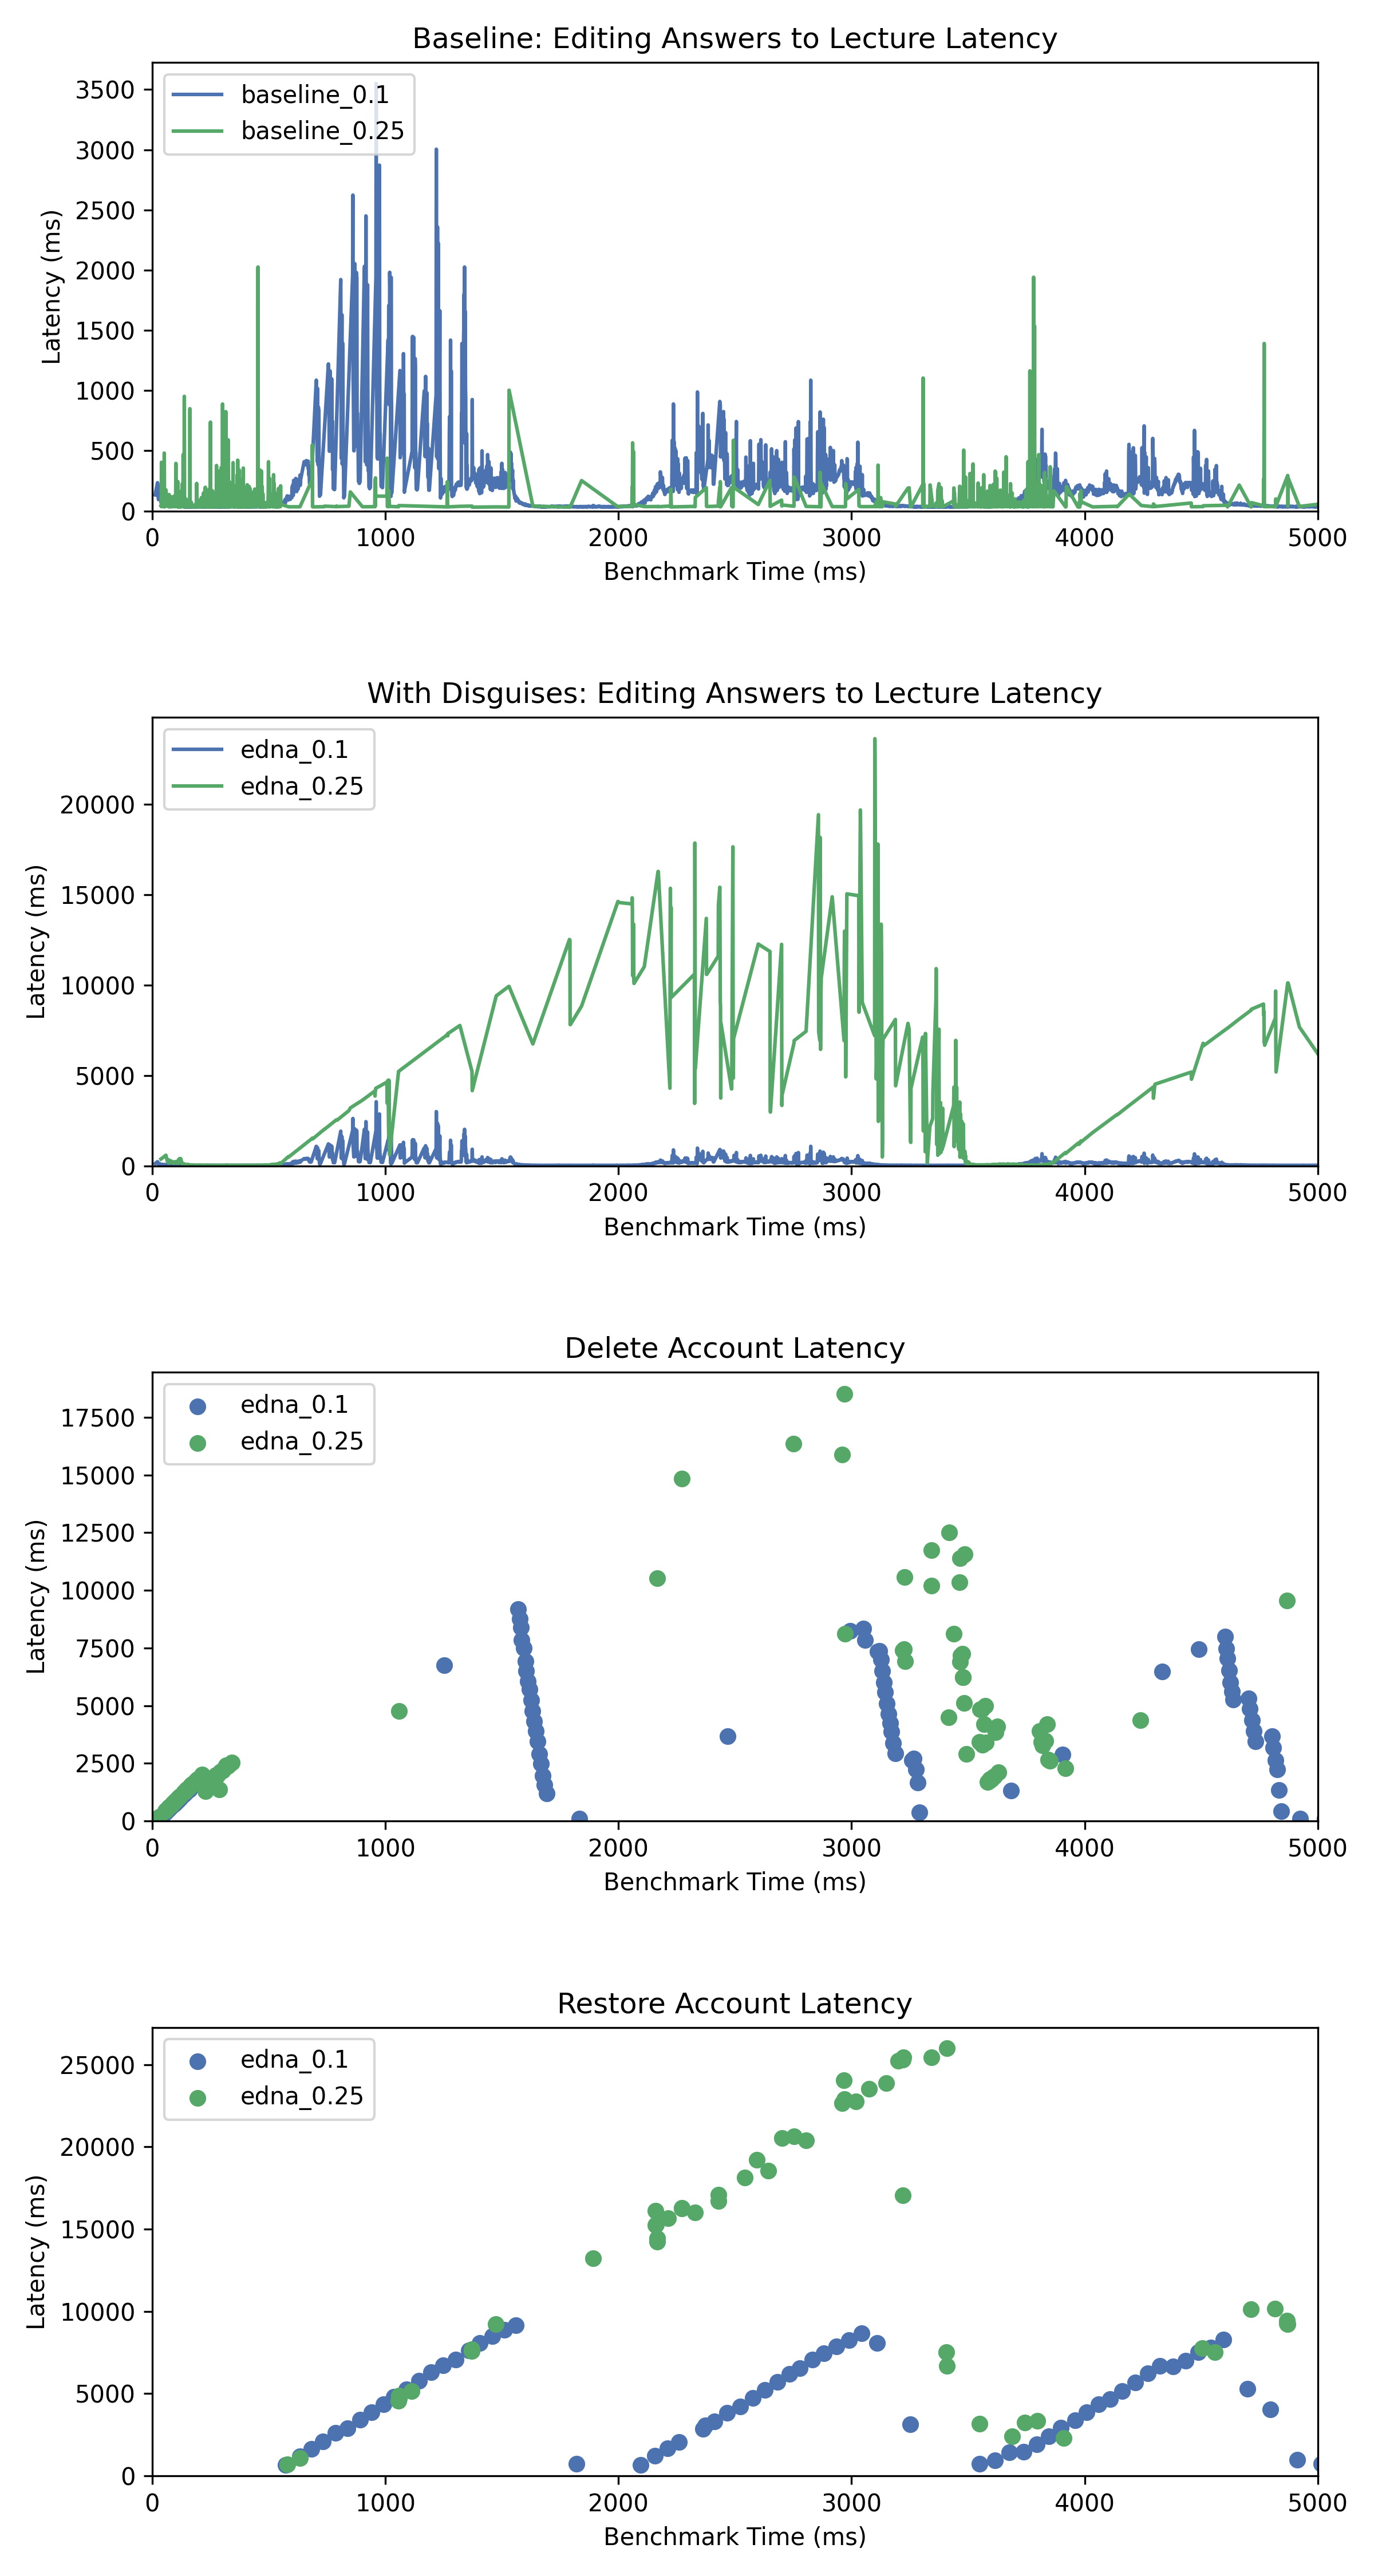
\includegraphics[width=0.45\textwidth]{figs/concurrent_results_40lec_200users}
    \caption{100 Users (left), 200 users (right); 
    40 lectures; 4 questions/lecture; ~5s sleep between disguise and reveal. }
\end{figure*}


